% Created by tikzDevice version 0.12.6 on 2025-09-19 10:58:40
% !TEX encoding = UTF-8 Unicode
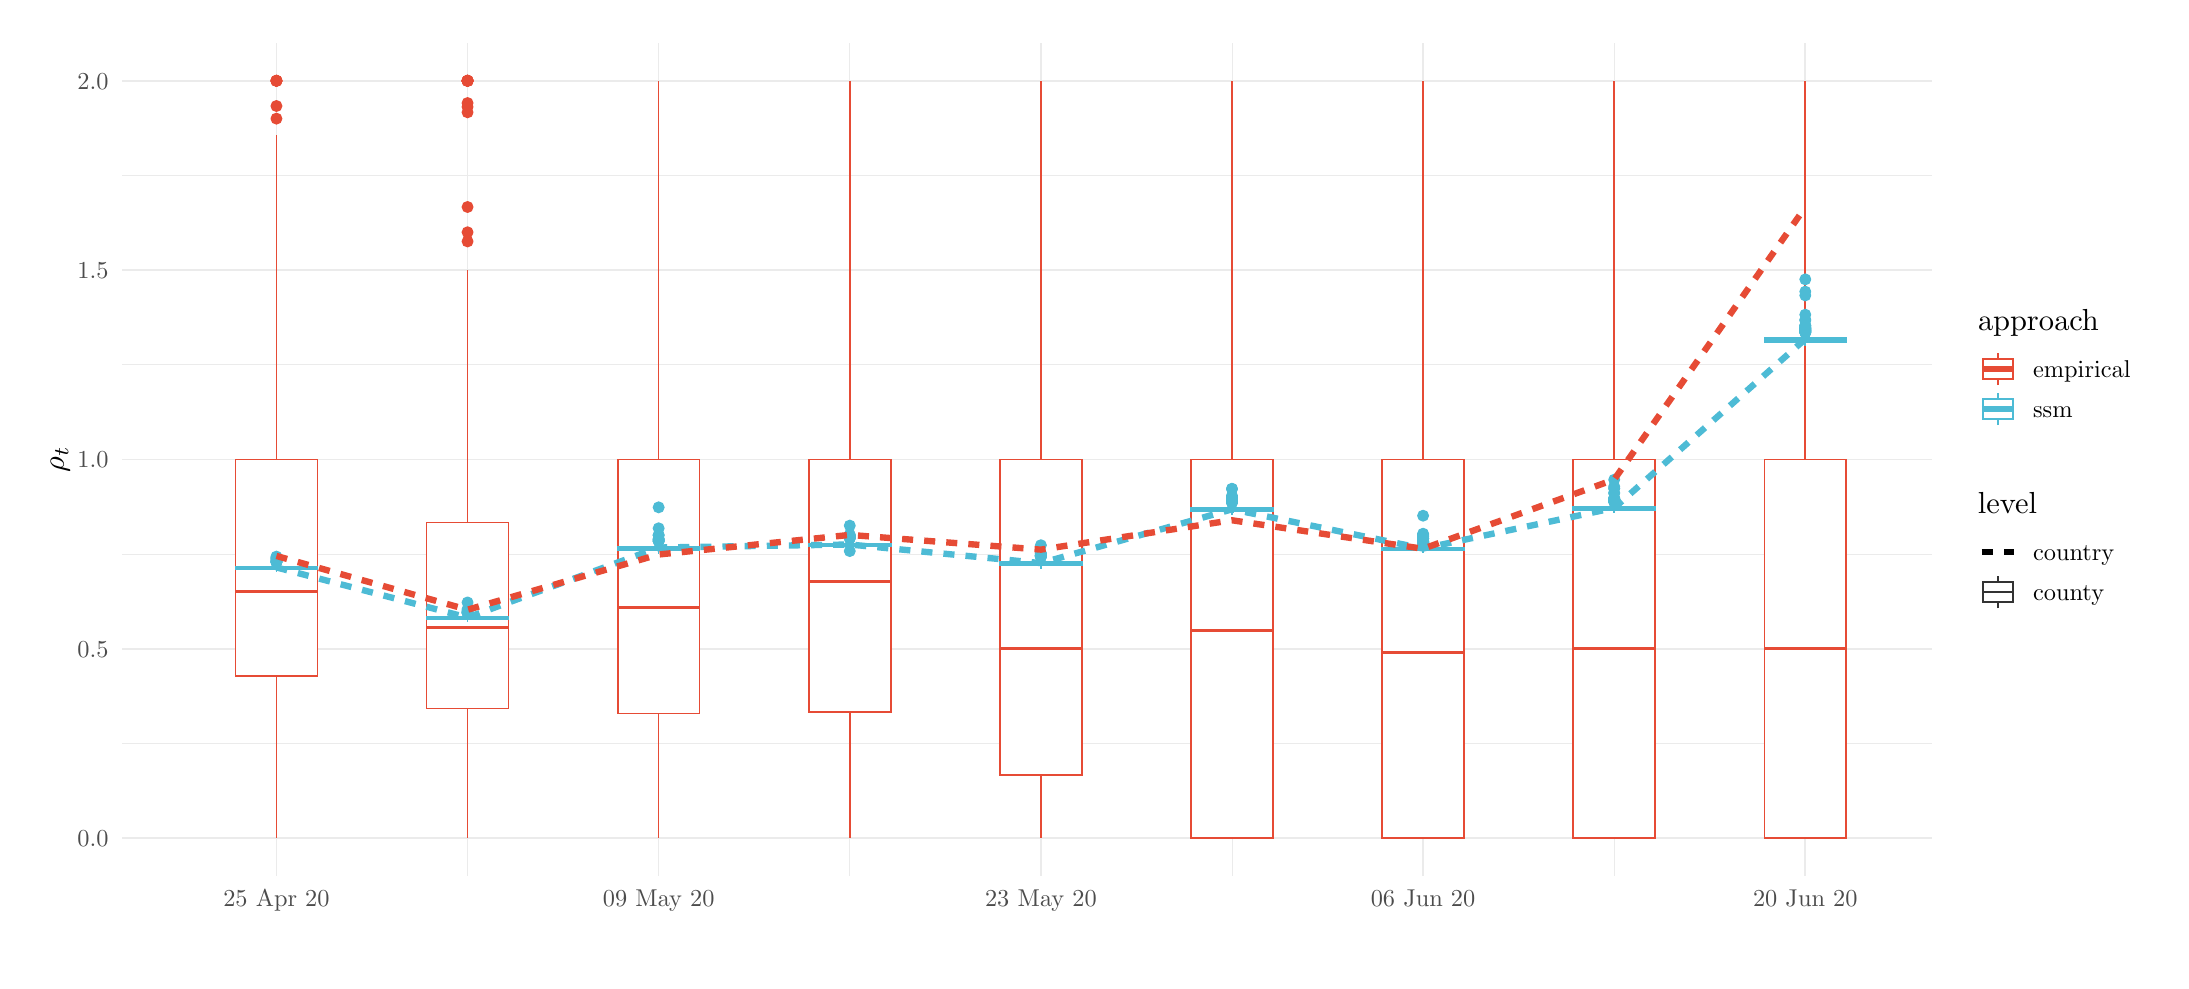
\begin{tikzpicture}[x=1pt,y=1pt]
\definecolor{fillColor}{RGB}{255,255,255}
\path[use as bounding box,fill=fillColor,fill opacity=0.00] (0,0) rectangle (770.88,337.26);
\begin{scope}
\path[clip] ( 34.16, 30.69) rectangle (688.21,331.76);
\definecolor{drawColor}{gray}{0.92}

\path[draw=drawColor,line width= 0.3pt,line join=round] ( 34.16, 78.58) --
	(688.21, 78.58);

\path[draw=drawColor,line width= 0.3pt,line join=round] ( 34.16,147.01) --
	(688.21,147.01);

\path[draw=drawColor,line width= 0.3pt,line join=round] ( 34.16,215.44) --
	(688.21,215.44);

\path[draw=drawColor,line width= 0.3pt,line join=round] ( 34.16,283.86) --
	(688.21,283.86);

\path[draw=drawColor,line width= 0.3pt,line join=round] (158.95, 30.69) --
	(158.95,331.76);

\path[draw=drawColor,line width= 0.3pt,line join=round] (297.06, 30.69) --
	(297.06,331.76);

\path[draw=drawColor,line width= 0.3pt,line join=round] (435.17, 30.69) --
	(435.17,331.76);

\path[draw=drawColor,line width= 0.3pt,line join=round] (573.28, 30.69) --
	(573.28,331.76);

\path[draw=drawColor,line width= 0.6pt,line join=round] ( 34.16, 44.37) --
	(688.21, 44.37);

\path[draw=drawColor,line width= 0.6pt,line join=round] ( 34.16,112.80) --
	(688.21,112.80);

\path[draw=drawColor,line width= 0.6pt,line join=round] ( 34.16,181.22) --
	(688.21,181.22);

\path[draw=drawColor,line width= 0.6pt,line join=round] ( 34.16,249.65) --
	(688.21,249.65);

\path[draw=drawColor,line width= 0.6pt,line join=round] ( 34.16,318.07) --
	(688.21,318.07);

\path[draw=drawColor,line width= 0.6pt,line join=round] ( 89.89, 30.69) --
	( 89.89,331.76);

\path[draw=drawColor,line width= 0.6pt,line join=round] (228.00, 30.69) --
	(228.00,331.76);

\path[draw=drawColor,line width= 0.6pt,line join=round] (366.12, 30.69) --
	(366.12,331.76);

\path[draw=drawColor,line width= 0.6pt,line join=round] (504.23, 30.69) --
	(504.23,331.76);

\path[draw=drawColor,line width= 0.6pt,line join=round] (642.34, 30.69) --
	(642.34,331.76);
\definecolor{drawColor}{RGB}{230,75,53}
\definecolor{fillColor}{RGB}{230,75,53}

\path[draw=drawColor,line width= 0.4pt,line join=round,line cap=round,fill=fillColor] ( 89.89,318.07) circle (  1.96);

\path[draw=drawColor,line width= 0.4pt,line join=round,line cap=round,fill=fillColor] ( 89.89,318.07) circle (  1.96);

\path[draw=drawColor,line width= 0.4pt,line join=round,line cap=round,fill=fillColor] ( 89.89,318.07) circle (  1.96);

\path[draw=drawColor,line width= 0.4pt,line join=round,line cap=round,fill=fillColor] ( 89.89,304.39) circle (  1.96);

\path[draw=drawColor,line width= 0.4pt,line join=round,line cap=round,fill=fillColor] ( 89.89,308.95) circle (  1.96);

\path[draw=drawColor,line width= 0.4pt,line join=round,line cap=round,fill=fillColor] ( 89.89,318.07) circle (  1.96);

\path[draw=drawColor,line width= 0.4pt,line join=round,line cap=round,fill=fillColor] ( 89.89,318.07) circle (  1.96);

\path[draw=drawColor,line width= 0.6pt,line join=round] ( 89.89,181.22) -- ( 89.89,298.52);

\path[draw=drawColor,line width= 0.6pt,line join=round] ( 89.89,103.02) -- ( 89.89, 44.37);
\definecolor{fillColor}{RGB}{255,255,255}

\path[draw=drawColor,line width= 0.6pt,fill=fillColor] ( 75.10,181.22) --
	( 75.10,103.02) --
	(104.69,103.02) --
	(104.69,181.22) --
	( 75.10,181.22) --
	cycle;

\path[draw=drawColor,line width= 1.1pt] ( 75.10,133.69) -- (104.69,133.69);
\definecolor{fillColor}{RGB}{230,75,53}

\path[draw=drawColor,line width= 0.4pt,line join=round,line cap=round,fill=fillColor] (158.95,318.07) circle (  1.96);

\path[draw=drawColor,line width= 0.4pt,line join=round,line cap=round,fill=fillColor] (158.95,272.46) circle (  1.96);

\path[draw=drawColor,line width= 0.4pt,line join=round,line cap=round,fill=fillColor] (158.95,263.33) circle (  1.96);

\path[draw=drawColor,line width= 0.4pt,line join=round,line cap=round,fill=fillColor] (158.95,310.02) circle (  1.96);

\path[draw=drawColor,line width= 0.4pt,line join=round,line cap=round,fill=fillColor] (158.95,260.02) circle (  1.96);

\path[draw=drawColor,line width= 0.4pt,line join=round,line cap=round,fill=fillColor] (158.95,306.67) circle (  1.96);

\path[draw=drawColor,line width= 0.4pt,line join=round,line cap=round,fill=fillColor] (158.95,318.07) circle (  1.96);

\path[draw=drawColor,line width= 0.4pt,line join=round,line cap=round,fill=fillColor] (158.95,308.64) circle (  1.96);

\path[draw=drawColor,line width= 0.4pt,line join=round,line cap=round,fill=fillColor] (158.95,318.07) circle (  1.96);

\path[draw=drawColor,line width= 0.4pt,line join=round,line cap=round,fill=fillColor] (158.95,318.07) circle (  1.96);

\path[draw=drawColor,line width= 0.4pt,line join=round,line cap=round,fill=fillColor] (158.95,318.07) circle (  1.96);

\path[draw=drawColor,line width= 0.4pt,line join=round,line cap=round,fill=fillColor] (158.95,318.07) circle (  1.96);

\path[draw=drawColor,line width= 0.4pt,line join=round,line cap=round,fill=fillColor] (158.95,318.07) circle (  1.96);

\path[draw=drawColor,line width= 0.4pt,line join=round,line cap=round,fill=fillColor] (158.95,318.07) circle (  1.96);

\path[draw=drawColor,line width= 0.6pt,line join=round] (158.95,158.41) -- (158.95,249.65);

\path[draw=drawColor,line width= 0.6pt,line join=round] (158.95, 91.19) -- (158.95, 44.37);
\definecolor{fillColor}{RGB}{255,255,255}

\path[draw=drawColor,line width= 0.6pt,fill=fillColor] (144.15,158.41) --
	(144.15, 91.19) --
	(173.75, 91.19) --
	(173.75,158.41) --
	(144.15,158.41) --
	cycle;

\path[draw=drawColor,line width= 1.1pt] (144.15,120.40) -- (173.75,120.40);

\path[draw=drawColor,line width= 0.6pt,line join=round] (228.00,181.22) -- (228.00,318.07);

\path[draw=drawColor,line width= 0.6pt,line join=round] (228.00, 89.40) -- (228.00, 44.37);

\path[draw=drawColor,line width= 0.6pt,fill=fillColor] (213.21,181.22) --
	(213.21, 89.40) --
	(242.80, 89.40) --
	(242.80,181.22) --
	(213.21,181.22) --
	cycle;

\path[draw=drawColor,line width= 1.1pt] (213.21,127.84) -- (242.80,127.84);

\path[draw=drawColor,line width= 0.6pt,line join=round] (297.06,181.22) -- (297.06,318.07);

\path[draw=drawColor,line width= 0.6pt,line join=round] (297.06, 89.99) -- (297.06, 44.37);

\path[draw=drawColor,line width= 0.6pt,fill=fillColor] (282.26,181.22) --
	(282.26, 89.99) --
	(311.86, 89.99) --
	(311.86,181.22) --
	(282.26,181.22) --
	cycle;

\path[draw=drawColor,line width= 1.1pt] (282.26,137.15) -- (311.86,137.15);

\path[draw=drawColor,line width= 0.6pt,line join=round] (366.12,181.22) -- (366.12,318.07);

\path[draw=drawColor,line width= 0.6pt,line join=round] (366.12, 67.18) -- (366.12, 44.37);

\path[draw=drawColor,line width= 0.6pt,fill=fillColor] (351.32,181.22) --
	(351.32, 67.18) --
	(380.91, 67.18) --
	(380.91,181.22) --
	(351.32,181.22) --
	cycle;

\path[draw=drawColor,line width= 1.1pt] (351.32,112.80) -- (380.91,112.80);

\path[draw=drawColor,line width= 0.6pt,line join=round] (435.17,181.22) -- (435.17,318.07);

\path[draw=drawColor,line width= 0.6pt,line join=round] (435.17, 44.37) -- (435.17, 44.37);

\path[draw=drawColor,line width= 0.6pt,fill=fillColor] (420.37,181.22) --
	(420.37, 44.37) --
	(449.97, 44.37) --
	(449.97,181.22) --
	(420.37,181.22) --
	cycle;

\path[draw=drawColor,line width= 1.1pt] (420.37,119.53) -- (449.97,119.53);

\path[draw=drawColor,line width= 0.6pt,line join=round] (504.23,181.22) -- (504.23,318.07);

\path[draw=drawColor,line width= 0.6pt,line join=round] (504.23, 44.37) -- (504.23, 44.37);

\path[draw=drawColor,line width= 0.6pt,fill=fillColor] (489.43,181.22) --
	(489.43, 44.37) --
	(519.02, 44.37) --
	(519.02,181.22) --
	(489.43,181.22) --
	cycle;

\path[draw=drawColor,line width= 1.1pt] (489.43,111.31) -- (519.02,111.31);

\path[draw=drawColor,line width= 0.6pt,line join=round] (573.28,181.22) -- (573.28,318.07);

\path[draw=drawColor,line width= 0.6pt,line join=round] (573.28, 44.37) -- (573.28, 44.37);

\path[draw=drawColor,line width= 0.6pt,fill=fillColor] (558.48,181.22) --
	(558.48, 44.37) --
	(588.08, 44.37) --
	(588.08,181.22) --
	(558.48,181.22) --
	cycle;

\path[draw=drawColor,line width= 1.1pt] (558.48,112.80) -- (588.08,112.80);

\path[draw=drawColor,line width= 0.6pt,line join=round] (642.34,181.22) -- (642.34,318.07);

\path[draw=drawColor,line width= 0.6pt,line join=round] (642.34, 44.37) -- (642.34, 44.37);

\path[draw=drawColor,line width= 0.6pt,fill=fillColor] (627.54,181.22) --
	(627.54, 44.37) --
	(657.14, 44.37) --
	(657.14,181.22) --
	(627.54,181.22) --
	cycle;

\path[draw=drawColor,line width= 1.1pt] (627.54,112.80) -- (657.14,112.80);
\definecolor{drawColor}{RGB}{77,187,213}
\definecolor{fillColor}{RGB}{77,187,213}

\path[draw=drawColor,line width= 0.4pt,line join=round,line cap=round,fill=fillColor] ( 89.89,145.80) circle (  1.96);

\path[draw=drawColor,line width= 0.4pt,line join=round,line cap=round,fill=fillColor] ( 89.89,146.13) circle (  1.96);

\path[draw=drawColor,line width= 0.4pt,line join=round,line cap=round,fill=fillColor] ( 89.89,145.05) circle (  1.96);

\path[draw=drawColor,line width= 0.4pt,line join=round,line cap=round,fill=fillColor] ( 89.89,144.66) circle (  1.96);

\path[draw=drawColor,line width= 0.4pt,line join=round,line cap=round,fill=fillColor] ( 89.89,144.55) circle (  1.96);

\path[draw=drawColor,line width= 0.4pt,line join=round,line cap=round,fill=fillColor] ( 89.89,145.46) circle (  1.96);

\path[draw=drawColor,line width= 0.4pt,line join=round,line cap=round,fill=fillColor] ( 89.89,144.15) circle (  1.96);

\path[draw=drawColor,line width= 0.4pt,line join=round,line cap=round,fill=fillColor] ( 89.89,144.16) circle (  1.96);

\path[draw=drawColor,line width= 0.4pt,line join=round,line cap=round,fill=fillColor] ( 89.89,144.06) circle (  1.96);

\path[draw=drawColor,line width= 0.4pt,line join=round,line cap=round,fill=fillColor] ( 89.89,144.27) circle (  1.96);

\path[draw=drawColor,line width= 0.4pt,line join=round,line cap=round,fill=fillColor] ( 89.89,145.44) circle (  1.96);

\path[draw=drawColor,line width= 0.4pt,line join=round,line cap=round,fill=fillColor] ( 89.89,144.31) circle (  1.96);

\path[draw=drawColor,line width= 0.6pt,line join=round] ( 89.89,142.61) -- ( 89.89,143.88);

\path[draw=drawColor,line width= 0.6pt,line join=round] ( 89.89,141.72) -- ( 89.89,140.72);
\definecolor{fillColor}{RGB}{255,255,255}

\path[draw=drawColor,line width= 0.6pt,fill=fillColor] ( 75.10,142.61) --
	( 75.10,141.72) --
	(104.69,141.72) --
	(104.69,142.61) --
	( 75.10,142.61) --
	cycle;

\path[draw=drawColor,line width= 1.1pt] ( 75.10,142.10) -- (104.69,142.10);
\definecolor{fillColor}{RGB}{77,187,213}

\path[draw=drawColor,line width= 0.4pt,line join=round,line cap=round,fill=fillColor] (158.95,129.56) circle (  1.96);

\path[draw=drawColor,line width= 0.4pt,line join=round,line cap=round,fill=fillColor] (158.95,126.56) circle (  1.96);

\path[draw=drawColor,line width= 0.4pt,line join=round,line cap=round,fill=fillColor] (158.95,125.88) circle (  1.96);

\path[draw=drawColor,line width= 0.4pt,line join=round,line cap=round,fill=fillColor] (158.95,126.26) circle (  1.96);

\path[draw=drawColor,line width= 0.4pt,line join=round,line cap=round,fill=fillColor] (158.95,127.16) circle (  1.96);

\path[draw=drawColor,line width= 0.4pt,line join=round,line cap=round,fill=fillColor] (158.95,125.97) circle (  1.96);

\path[draw=drawColor,line width= 0.4pt,line join=round,line cap=round,fill=fillColor] (158.95,125.63) circle (  1.96);

\path[draw=drawColor,line width= 0.4pt,line join=round,line cap=round,fill=fillColor] (158.95,125.90) circle (  1.96);

\path[draw=drawColor,line width= 0.6pt,line join=round] (158.95,124.40) -- (158.95,125.56);

\path[draw=drawColor,line width= 0.6pt,line join=round] (158.95,123.60) -- (158.95,122.61);
\definecolor{fillColor}{RGB}{255,255,255}

\path[draw=drawColor,line width= 0.6pt,fill=fillColor] (144.15,124.40) --
	(144.15,123.60) --
	(173.75,123.60) --
	(173.75,124.40) --
	(144.15,124.40) --
	cycle;

\path[draw=drawColor,line width= 1.1pt] (144.15,124.01) -- (173.75,124.01);
\definecolor{fillColor}{RGB}{77,187,213}

\path[draw=drawColor,line width= 0.4pt,line join=round,line cap=round,fill=fillColor] (228.00,151.77) circle (  1.96);

\path[draw=drawColor,line width= 0.4pt,line join=round,line cap=round,fill=fillColor] (228.00,163.93) circle (  1.96);

\path[draw=drawColor,line width= 0.4pt,line join=round,line cap=round,fill=fillColor] (228.00,153.95) circle (  1.96);

\path[draw=drawColor,line width= 0.4pt,line join=round,line cap=round,fill=fillColor] (228.00,151.67) circle (  1.96);

\path[draw=drawColor,line width= 0.4pt,line join=round,line cap=round,fill=fillColor] (228.00,152.63) circle (  1.96);

\path[draw=drawColor,line width= 0.4pt,line join=round,line cap=round,fill=fillColor] (228.00,152.31) circle (  1.96);

\path[draw=drawColor,line width= 0.4pt,line join=round,line cap=round,fill=fillColor] (228.00,152.21) circle (  1.96);

\path[draw=drawColor,line width= 0.4pt,line join=round,line cap=round,fill=fillColor] (228.00,156.36) circle (  1.96);

\path[draw=drawColor,line width= 0.4pt,line join=round,line cap=round,fill=fillColor] (228.00,153.82) circle (  1.96);

\path[draw=drawColor,line width= 0.4pt,line join=round,line cap=round,fill=fillColor] (228.00,151.73) circle (  1.96);

\path[draw=drawColor,line width= 0.6pt,line join=round] (228.00,149.84) -- (228.00,151.56);

\path[draw=drawColor,line width= 0.6pt,line join=round] (228.00,148.62) -- (228.00,147.17);
\definecolor{fillColor}{RGB}{255,255,255}

\path[draw=drawColor,line width= 0.6pt,fill=fillColor] (213.21,149.84) --
	(213.21,148.62) --
	(242.80,148.62) --
	(242.80,149.84) --
	(213.21,149.84) --
	cycle;

\path[draw=drawColor,line width= 1.1pt] (213.21,149.24) -- (242.80,149.24);
\definecolor{fillColor}{RGB}{77,187,213}

\path[draw=drawColor,line width= 0.4pt,line join=round,line cap=round,fill=fillColor] (297.06,153.52) circle (  1.96);

\path[draw=drawColor,line width= 0.4pt,line join=round,line cap=round,fill=fillColor] (297.06,157.33) circle (  1.96);

\path[draw=drawColor,line width= 0.4pt,line join=round,line cap=round,fill=fillColor] (297.06,152.82) circle (  1.96);

\path[draw=drawColor,line width= 0.4pt,line join=round,line cap=round,fill=fillColor] (297.06,153.50) circle (  1.96);

\path[draw=drawColor,line width= 0.4pt,line join=round,line cap=round,fill=fillColor] (297.06,153.23) circle (  1.96);

\path[draw=drawColor,line width= 0.4pt,line join=round,line cap=round,fill=fillColor] (297.06,153.25) circle (  1.96);

\path[draw=drawColor,line width= 0.4pt,line join=round,line cap=round,fill=fillColor] (297.06,153.18) circle (  1.96);

\path[draw=drawColor,line width= 0.4pt,line join=round,line cap=round,fill=fillColor] (297.06,154.12) circle (  1.96);

\path[draw=drawColor,line width= 0.4pt,line join=round,line cap=round,fill=fillColor] (297.06,153.64) circle (  1.96);

\path[draw=drawColor,line width= 0.4pt,line join=round,line cap=round,fill=fillColor] (297.06,152.68) circle (  1.96);

\path[draw=drawColor,line width= 0.4pt,line join=round,line cap=round,fill=fillColor] (297.06,153.56) circle (  1.96);

\path[draw=drawColor,line width= 0.4pt,line join=round,line cap=round,fill=fillColor] (297.06,153.39) circle (  1.96);

\path[draw=drawColor,line width= 0.4pt,line join=round,line cap=round,fill=fillColor] (297.06,153.42) circle (  1.96);

\path[draw=drawColor,line width= 0.4pt,line join=round,line cap=round,fill=fillColor] (297.06,152.79) circle (  1.96);

\path[draw=drawColor,line width= 0.4pt,line join=round,line cap=round,fill=fillColor] (297.06,148.13) circle (  1.96);

\path[draw=drawColor,line width= 0.6pt,line join=round] (297.06,150.90) -- (297.06,152.48);

\path[draw=drawColor,line width= 0.6pt,line join=round] (297.06,149.80) -- (297.06,148.48);
\definecolor{fillColor}{RGB}{255,255,255}

\path[draw=drawColor,line width= 0.6pt,fill=fillColor] (282.26,150.90) --
	(282.26,149.80) --
	(311.86,149.80) --
	(311.86,150.90) --
	(282.26,150.90) --
	cycle;

\path[draw=drawColor,line width= 1.1pt] (282.26,150.32) -- (311.86,150.32);
\definecolor{fillColor}{RGB}{77,187,213}

\path[draw=drawColor,line width= 0.4pt,line join=round,line cap=round,fill=fillColor] (366.12,146.43) circle (  1.96);

\path[draw=drawColor,line width= 0.4pt,line join=round,line cap=round,fill=fillColor] (366.12,150.25) circle (  1.96);

\path[draw=drawColor,line width= 0.4pt,line join=round,line cap=round,fill=fillColor] (366.12,146.89) circle (  1.96);

\path[draw=drawColor,line width= 0.4pt,line join=round,line cap=round,fill=fillColor] (366.12,147.28) circle (  1.96);

\path[draw=drawColor,line width= 0.4pt,line join=round,line cap=round,fill=fillColor] (366.12,146.37) circle (  1.96);

\path[draw=drawColor,line width= 0.4pt,line join=round,line cap=round,fill=fillColor] (366.12,146.59) circle (  1.96);

\path[draw=drawColor,line width= 0.4pt,line join=round,line cap=round,fill=fillColor] (366.12,147.06) circle (  1.96);

\path[draw=drawColor,line width= 0.4pt,line join=round,line cap=round,fill=fillColor] (366.12,147.22) circle (  1.96);

\path[draw=drawColor,line width= 0.4pt,line join=round,line cap=round,fill=fillColor] (366.12,146.51) circle (  1.96);

\path[draw=drawColor,line width= 0.4pt,line join=round,line cap=round,fill=fillColor] (366.12,146.58) circle (  1.96);

\path[draw=drawColor,line width= 0.4pt,line join=round,line cap=round,fill=fillColor] (366.12,146.35) circle (  1.96);

\path[draw=drawColor,line width= 0.4pt,line join=round,line cap=round,fill=fillColor] (366.12,146.64) circle (  1.96);

\path[draw=drawColor,line width= 0.4pt,line join=round,line cap=round,fill=fillColor] (366.12,145.98) circle (  1.96);

\path[draw=drawColor,line width= 0.4pt,line join=round,line cap=round,fill=fillColor] (366.12,146.07) circle (  1.96);

\path[draw=drawColor,line width= 0.4pt,line join=round,line cap=round,fill=fillColor] (366.12,146.16) circle (  1.96);

\path[draw=drawColor,line width= 0.4pt,line join=round,line cap=round,fill=fillColor] (366.12,146.50) circle (  1.96);

\path[draw=drawColor,line width= 0.4pt,line join=round,line cap=round,fill=fillColor] (366.12,146.33) circle (  1.96);

\path[draw=drawColor,line width= 0.6pt,line join=round] (366.12,144.19) -- (366.12,145.74);

\path[draw=drawColor,line width= 0.6pt,line join=round] (366.12,143.09) -- (366.12,141.78);
\definecolor{fillColor}{RGB}{255,255,255}

\path[draw=drawColor,line width= 0.6pt,fill=fillColor] (351.32,144.19) --
	(351.32,143.09) --
	(380.91,143.09) --
	(380.91,144.19) --
	(351.32,144.19) --
	cycle;

\path[draw=drawColor,line width= 1.1pt] (351.32,143.56) -- (380.91,143.56);
\definecolor{fillColor}{RGB}{77,187,213}

\path[draw=drawColor,line width= 0.4pt,line join=round,line cap=round,fill=fillColor] (435.17,166.29) circle (  1.96);

\path[draw=drawColor,line width= 0.4pt,line join=round,line cap=round,fill=fillColor] (435.17,166.86) circle (  1.96);

\path[draw=drawColor,line width= 0.4pt,line join=round,line cap=round,fill=fillColor] (435.17,166.02) circle (  1.96);

\path[draw=drawColor,line width= 0.4pt,line join=round,line cap=round,fill=fillColor] (435.17,170.66) circle (  1.96);

\path[draw=drawColor,line width= 0.4pt,line join=round,line cap=round,fill=fillColor] (435.17,166.63) circle (  1.96);

\path[draw=drawColor,line width= 0.4pt,line join=round,line cap=round,fill=fillColor] (435.17,166.23) circle (  1.96);

\path[draw=drawColor,line width= 0.4pt,line join=round,line cap=round,fill=fillColor] (435.17,168.14) circle (  1.96);

\path[draw=drawColor,line width= 0.4pt,line join=round,line cap=round,fill=fillColor] (435.17,165.80) circle (  1.96);

\path[draw=drawColor,line width= 0.4pt,line join=round,line cap=round,fill=fillColor] (435.17,167.38) circle (  1.96);

\path[draw=drawColor,line width= 0.4pt,line join=round,line cap=round,fill=fillColor] (435.17,170.55) circle (  1.96);

\path[draw=drawColor,line width= 0.4pt,line join=round,line cap=round,fill=fillColor] (435.17,165.64) circle (  1.96);

\path[draw=drawColor,line width= 0.4pt,line join=round,line cap=round,fill=fillColor] (435.17,167.34) circle (  1.96);

\path[draw=drawColor,line width= 0.4pt,line join=round,line cap=round,fill=fillColor] (435.17,165.86) circle (  1.96);

\path[draw=drawColor,line width= 0.4pt,line join=round,line cap=round,fill=fillColor] (435.17,166.78) circle (  1.96);

\path[draw=drawColor,line width= 0.4pt,line join=round,line cap=round,fill=fillColor] (435.17,166.09) circle (  1.96);

\path[draw=drawColor,line width= 0.4pt,line join=round,line cap=round,fill=fillColor] (435.17,166.13) circle (  1.96);

\path[draw=drawColor,line width= 0.4pt,line join=round,line cap=round,fill=fillColor] (435.17,166.90) circle (  1.96);

\path[draw=drawColor,line width= 0.4pt,line join=round,line cap=round,fill=fillColor] (435.17,165.64) circle (  1.96);

\path[draw=drawColor,line width= 0.4pt,line join=round,line cap=round,fill=fillColor] (435.17,166.25) circle (  1.96);

\path[draw=drawColor,line width= 0.6pt,line join=round] (435.17,163.75) -- (435.17,165.36);

\path[draw=drawColor,line width= 0.6pt,line join=round] (435.17,162.60) -- (435.17,161.24);
\definecolor{fillColor}{RGB}{255,255,255}

\path[draw=drawColor,line width= 0.6pt,fill=fillColor] (420.37,163.75) --
	(420.37,162.60) --
	(449.97,162.60) --
	(449.97,163.75) --
	(420.37,163.75) --
	cycle;

\path[draw=drawColor,line width= 1.1pt] (420.37,163.05) -- (449.97,163.05);
\definecolor{fillColor}{RGB}{77,187,213}

\path[draw=drawColor,line width= 0.4pt,line join=round,line cap=round,fill=fillColor] (504.23,151.67) circle (  1.96);

\path[draw=drawColor,line width= 0.4pt,line join=round,line cap=round,fill=fillColor] (504.23,152.68) circle (  1.96);

\path[draw=drawColor,line width= 0.4pt,line join=round,line cap=round,fill=fillColor] (504.23,160.91) circle (  1.96);

\path[draw=drawColor,line width= 0.4pt,line join=round,line cap=round,fill=fillColor] (504.23,151.22) circle (  1.96);

\path[draw=drawColor,line width= 0.4pt,line join=round,line cap=round,fill=fillColor] (504.23,151.27) circle (  1.96);

\path[draw=drawColor,line width= 0.4pt,line join=round,line cap=round,fill=fillColor] (504.23,152.07) circle (  1.96);

\path[draw=drawColor,line width= 0.4pt,line join=round,line cap=round,fill=fillColor] (504.23,153.38) circle (  1.96);

\path[draw=drawColor,line width= 0.4pt,line join=round,line cap=round,fill=fillColor] (504.23,151.16) circle (  1.96);

\path[draw=drawColor,line width= 0.4pt,line join=round,line cap=round,fill=fillColor] (504.23,150.87) circle (  1.96);

\path[draw=drawColor,line width= 0.4pt,line join=round,line cap=round,fill=fillColor] (504.23,150.98) circle (  1.96);

\path[draw=drawColor,line width= 0.4pt,line join=round,line cap=round,fill=fillColor] (504.23,152.86) circle (  1.96);

\path[draw=drawColor,line width= 0.4pt,line join=round,line cap=round,fill=fillColor] (504.23,154.40) circle (  1.96);

\path[draw=drawColor,line width= 0.4pt,line join=round,line cap=round,fill=fillColor] (504.23,153.73) circle (  1.96);

\path[draw=drawColor,line width= 0.4pt,line join=round,line cap=round,fill=fillColor] (504.23,151.10) circle (  1.96);

\path[draw=drawColor,line width= 0.4pt,line join=round,line cap=round,fill=fillColor] (504.23,151.52) circle (  1.96);

\path[draw=drawColor,line width= 0.4pt,line join=round,line cap=round,fill=fillColor] (504.23,151.45) circle (  1.96);

\path[draw=drawColor,line width= 0.4pt,line join=round,line cap=round,fill=fillColor] (504.23,151.45) circle (  1.96);

\path[draw=drawColor,line width= 0.4pt,line join=round,line cap=round,fill=fillColor] (504.23,154.07) circle (  1.96);

\path[draw=drawColor,line width= 0.4pt,line join=round,line cap=round,fill=fillColor] (504.23,151.57) circle (  1.96);

\path[draw=drawColor,line width= 0.4pt,line join=round,line cap=round,fill=fillColor] (504.23,151.20) circle (  1.96);

\path[draw=drawColor,line width= 0.4pt,line join=round,line cap=round,fill=fillColor] (504.23,152.68) circle (  1.96);

\path[draw=drawColor,line width= 0.6pt,line join=round] (504.23,149.40) -- (504.23,150.84);

\path[draw=drawColor,line width= 0.6pt,line join=round] (504.23,148.43) -- (504.23,147.26);
\definecolor{fillColor}{RGB}{255,255,255}

\path[draw=drawColor,line width= 0.6pt,fill=fillColor] (489.43,149.40) --
	(489.43,148.43) --
	(519.02,148.43) --
	(519.02,149.40) --
	(489.43,149.40) --
	cycle;

\path[draw=drawColor,line width= 1.1pt] (489.43,148.82) -- (519.02,148.82);
\definecolor{fillColor}{RGB}{77,187,213}

\path[draw=drawColor,line width= 0.4pt,line join=round,line cap=round,fill=fillColor] (573.28,166.61) circle (  1.96);

\path[draw=drawColor,line width= 0.4pt,line join=round,line cap=round,fill=fillColor] (573.28,165.91) circle (  1.96);

\path[draw=drawColor,line width= 0.4pt,line join=round,line cap=round,fill=fillColor] (573.28,170.78) circle (  1.96);

\path[draw=drawColor,line width= 0.4pt,line join=round,line cap=round,fill=fillColor] (573.28,166.46) circle (  1.96);

\path[draw=drawColor,line width= 0.4pt,line join=round,line cap=round,fill=fillColor] (573.28,166.35) circle (  1.96);

\path[draw=drawColor,line width= 0.4pt,line join=round,line cap=round,fill=fillColor] (573.28,170.74) circle (  1.96);

\path[draw=drawColor,line width= 0.4pt,line join=round,line cap=round,fill=fillColor] (573.28,173.91) circle (  1.96);

\path[draw=drawColor,line width= 0.4pt,line join=round,line cap=round,fill=fillColor] (573.28,166.12) circle (  1.96);

\path[draw=drawColor,line width= 0.4pt,line join=round,line cap=round,fill=fillColor] (573.28,167.32) circle (  1.96);

\path[draw=drawColor,line width= 0.4pt,line join=round,line cap=round,fill=fillColor] (573.28,166.77) circle (  1.96);

\path[draw=drawColor,line width= 0.4pt,line join=round,line cap=round,fill=fillColor] (573.28,166.15) circle (  1.96);

\path[draw=drawColor,line width= 0.4pt,line join=round,line cap=round,fill=fillColor] (573.28,165.96) circle (  1.96);

\path[draw=drawColor,line width= 0.4pt,line join=round,line cap=round,fill=fillColor] (573.28,169.15) circle (  1.96);

\path[draw=drawColor,line width= 0.4pt,line join=round,line cap=round,fill=fillColor] (573.28,167.15) circle (  1.96);

\path[draw=drawColor,line width= 0.4pt,line join=round,line cap=round,fill=fillColor] (573.28,166.55) circle (  1.96);

\path[draw=drawColor,line width= 0.4pt,line join=round,line cap=round,fill=fillColor] (573.28,169.04) circle (  1.96);

\path[draw=drawColor,line width= 0.4pt,line join=round,line cap=round,fill=fillColor] (573.28,171.49) circle (  1.96);

\path[draw=drawColor,line width= 0.4pt,line join=round,line cap=round,fill=fillColor] (573.28,167.16) circle (  1.96);

\path[draw=drawColor,line width= 0.6pt,line join=round] (573.28,164.18) -- (573.28,165.62);

\path[draw=drawColor,line width= 0.6pt,line join=round] (573.28,163.06) -- (573.28,161.94);
\definecolor{fillColor}{RGB}{255,255,255}

\path[draw=drawColor,line width= 0.6pt,fill=fillColor] (558.48,164.18) --
	(558.48,163.06) --
	(588.08,163.06) --
	(588.08,164.18) --
	(558.48,164.18) --
	cycle;

\path[draw=drawColor,line width= 1.1pt] (558.48,163.45) -- (588.08,163.45);
\definecolor{fillColor}{RGB}{77,187,213}

\path[draw=drawColor,line width= 0.4pt,line join=round,line cap=round,fill=fillColor] (642.34,227.23) circle (  1.96);

\path[draw=drawColor,line width= 0.4pt,line join=round,line cap=round,fill=fillColor] (642.34,227.20) circle (  1.96);

\path[draw=drawColor,line width= 0.4pt,line join=round,line cap=round,fill=fillColor] (642.34,231.77) circle (  1.96);

\path[draw=drawColor,line width= 0.4pt,line join=round,line cap=round,fill=fillColor] (642.34,229.36) circle (  1.96);

\path[draw=drawColor,line width= 0.4pt,line join=round,line cap=round,fill=fillColor] (642.34,240.51) circle (  1.96);

\path[draw=drawColor,line width= 0.4pt,line join=round,line cap=round,fill=fillColor] (642.34,228.29) circle (  1.96);

\path[draw=drawColor,line width= 0.4pt,line join=round,line cap=round,fill=fillColor] (642.34,246.31) circle (  1.96);

\path[draw=drawColor,line width= 0.4pt,line join=round,line cap=round,fill=fillColor] (642.34,227.67) circle (  1.96);

\path[draw=drawColor,line width= 0.4pt,line join=round,line cap=round,fill=fillColor] (642.34,228.28) circle (  1.96);

\path[draw=drawColor,line width= 0.4pt,line join=round,line cap=round,fill=fillColor] (642.34,228.79) circle (  1.96);

\path[draw=drawColor,line width= 0.4pt,line join=round,line cap=round,fill=fillColor] (642.34,231.43) circle (  1.96);

\path[draw=drawColor,line width= 0.4pt,line join=round,line cap=round,fill=fillColor] (642.34,227.64) circle (  1.96);

\path[draw=drawColor,line width= 0.4pt,line join=round,line cap=round,fill=fillColor] (642.34,228.15) circle (  1.96);

\path[draw=drawColor,line width= 0.4pt,line join=round,line cap=round,fill=fillColor] (642.34,228.74) circle (  1.96);

\path[draw=drawColor,line width= 0.4pt,line join=round,line cap=round,fill=fillColor] (642.34,227.17) circle (  1.96);

\path[draw=drawColor,line width= 0.4pt,line join=round,line cap=round,fill=fillColor] (642.34,227.60) circle (  1.96);

\path[draw=drawColor,line width= 0.4pt,line join=round,line cap=round,fill=fillColor] (642.34,227.12) circle (  1.96);

\path[draw=drawColor,line width= 0.4pt,line join=round,line cap=round,fill=fillColor] (642.34,228.52) circle (  1.96);

\path[draw=drawColor,line width= 0.4pt,line join=round,line cap=round,fill=fillColor] (642.34,228.17) circle (  1.96);

\path[draw=drawColor,line width= 0.4pt,line join=round,line cap=round,fill=fillColor] (642.34,227.84) circle (  1.96);

\path[draw=drawColor,line width= 0.4pt,line join=round,line cap=round,fill=fillColor] (642.34,227.58) circle (  1.96);

\path[draw=drawColor,line width= 0.4pt,line join=round,line cap=round,fill=fillColor] (642.34,229.65) circle (  1.96);

\path[draw=drawColor,line width= 0.4pt,line join=round,line cap=round,fill=fillColor] (642.34,227.89) circle (  1.96);

\path[draw=drawColor,line width= 0.4pt,line join=round,line cap=round,fill=fillColor] (642.34,227.90) circle (  1.96);

\path[draw=drawColor,line width= 0.4pt,line join=round,line cap=round,fill=fillColor] (642.34,229.60) circle (  1.96);

\path[draw=drawColor,line width= 0.4pt,line join=round,line cap=round,fill=fillColor] (642.34,228.67) circle (  1.96);

\path[draw=drawColor,line width= 0.4pt,line join=round,line cap=round,fill=fillColor] (642.34,227.22) circle (  1.96);

\path[draw=drawColor,line width= 0.4pt,line join=round,line cap=round,fill=fillColor] (642.34,229.48) circle (  1.96);

\path[draw=drawColor,line width= 0.4pt,line join=round,line cap=round,fill=fillColor] (642.34,227.12) circle (  1.96);

\path[draw=drawColor,line width= 0.4pt,line join=round,line cap=round,fill=fillColor] (642.34,241.88) circle (  1.96);

\path[draw=drawColor,line width= 0.4pt,line join=round,line cap=round,fill=fillColor] (642.34,228.09) circle (  1.96);

\path[draw=drawColor,line width= 0.4pt,line join=round,line cap=round,fill=fillColor] (642.34,228.72) circle (  1.96);

\path[draw=drawColor,line width= 0.4pt,line join=round,line cap=round,fill=fillColor] (642.34,233.55) circle (  1.96);

\path[draw=drawColor,line width= 0.6pt,line join=round] (642.34,225.08) -- (642.34,227.03);

\path[draw=drawColor,line width= 0.6pt,line join=round] (642.34,223.74) -- (642.34,222.29);
\definecolor{fillColor}{RGB}{255,255,255}

\path[draw=drawColor,line width= 0.6pt,fill=fillColor] (627.54,225.08) --
	(627.54,223.74) --
	(657.14,223.74) --
	(657.14,225.08) --
	(627.54,225.08) --
	cycle;

\path[draw=drawColor,line width= 1.1pt] (627.54,224.28) -- (657.14,224.28);

\path[draw=drawColor,line width= 2.3pt,dash pattern=on 4pt off 4pt ,line join=round] ( 89.89,142.22) --
	(158.95,124.12) --
	(228.00,149.41) --
	(297.06,150.50) --
	(366.12,143.78) --
	(435.17,163.21) --
	(504.23,149.06) --
	(573.28,163.70) --
	(642.34,224.74);
\definecolor{drawColor}{RGB}{230,75,53}

\path[draw=drawColor,line width= 2.3pt,dash pattern=on 4pt off 4pt ,line join=round] ( 89.89,146.36) --
	(158.95,126.93) --
	(228.00,146.89) --
	(297.06,153.97) --
	(366.12,148.65) --
	(435.17,159.26) --
	(504.23,148.96) --
	(573.28,173.97) --
	(642.34,272.38);
\end{scope}
\begin{scope}
\path[clip] (  0.00,  0.00) rectangle (770.88,337.26);
\definecolor{drawColor}{gray}{0.30}

\node[text=drawColor,anchor=base east,inner sep=0pt, outer sep=0pt, scale=  0.88] at ( 29.21, 41.34) {0.0};

\node[text=drawColor,anchor=base east,inner sep=0pt, outer sep=0pt, scale=  0.88] at ( 29.21,109.77) {0.5};

\node[text=drawColor,anchor=base east,inner sep=0pt, outer sep=0pt, scale=  0.88] at ( 29.21,178.19) {1.0};

\node[text=drawColor,anchor=base east,inner sep=0pt, outer sep=0pt, scale=  0.88] at ( 29.21,246.62) {1.5};

\node[text=drawColor,anchor=base east,inner sep=0pt, outer sep=0pt, scale=  0.88] at ( 29.21,315.04) {2.0};
\end{scope}
\begin{scope}
\path[clip] (  0.00,  0.00) rectangle (770.88,337.26);
\definecolor{drawColor}{gray}{0.30}

\node[text=drawColor,anchor=base,inner sep=0pt, outer sep=0pt, scale=  0.88] at ( 89.89, 19.68) {25 Apr 20};

\node[text=drawColor,anchor=base,inner sep=0pt, outer sep=0pt, scale=  0.88] at (228.00, 19.68) {09 May 20};

\node[text=drawColor,anchor=base,inner sep=0pt, outer sep=0pt, scale=  0.88] at (366.12, 19.68) {23 May 20};

\node[text=drawColor,anchor=base,inner sep=0pt, outer sep=0pt, scale=  0.88] at (504.23, 19.68) {06 Jun 20};

\node[text=drawColor,anchor=base,inner sep=0pt, outer sep=0pt, scale=  0.88] at (642.34, 19.68) {20 Jun 20};
\end{scope}
\begin{scope}
\path[clip] (  0.00,  0.00) rectangle (770.88,337.26);
\definecolor{drawColor}{RGB}{0,0,0}

\node[text=drawColor,rotate= 90.00,anchor=base,inner sep=0pt, outer sep=0pt, scale=  1.10] at ( 13.08,181.22) {$\rho_{t}$};
\end{scope}
\begin{scope}
\path[clip] (  0.00,  0.00) rectangle (770.88,337.26);
\definecolor{drawColor}{RGB}{0,0,0}

\node[text=drawColor,anchor=base west,inner sep=0pt, outer sep=0pt, scale=  1.10] at (704.71,227.70) {approach};
\end{scope}
\begin{scope}
\path[clip] (  0.00,  0.00) rectangle (770.88,337.26);
\definecolor{drawColor}{RGB}{230,75,53}

\path[draw=drawColor,line width= 0.6pt] (711.94,208.12) --
	(711.94,210.29);

\path[draw=drawColor,line width= 0.6pt] (711.94,217.52) --
	(711.94,219.69);
\definecolor{fillColor}{RGB}{255,255,255}

\path[draw=drawColor,line width= 0.6pt,fill=fillColor] (706.52,210.29) rectangle (717.36,217.52);

\path[draw=drawColor,line width= 0.6pt] (706.52,213.90) --
	(717.36,213.90);
\end{scope}
\begin{scope}
\path[clip] (  0.00,  0.00) rectangle (770.88,337.26);
\definecolor{drawColor}{RGB}{230,75,53}

\path[draw=drawColor,line width= 2.3pt,line join=round] (706.16,213.90) -- (717.72,213.90);
\end{scope}
\begin{scope}
\path[clip] (  0.00,  0.00) rectangle (770.88,337.26);
\definecolor{drawColor}{RGB}{77,187,213}

\path[draw=drawColor,line width= 0.6pt] (711.94,193.67) --
	(711.94,195.84);

\path[draw=drawColor,line width= 0.6pt] (711.94,203.06) --
	(711.94,205.23);
\definecolor{fillColor}{RGB}{255,255,255}

\path[draw=drawColor,line width= 0.6pt,fill=fillColor] (706.52,195.84) rectangle (717.36,203.06);

\path[draw=drawColor,line width= 0.6pt] (706.52,199.45) --
	(717.36,199.45);
\end{scope}
\begin{scope}
\path[clip] (  0.00,  0.00) rectangle (770.88,337.26);
\definecolor{drawColor}{RGB}{77,187,213}

\path[draw=drawColor,line width= 2.3pt,line join=round] (706.16,199.45) -- (717.72,199.45);
\end{scope}
\begin{scope}
\path[clip] (  0.00,  0.00) rectangle (770.88,337.26);
\definecolor{drawColor}{RGB}{0,0,0}

\node[text=drawColor,anchor=base west,inner sep=0pt, outer sep=0pt, scale=  0.88] at (724.66,210.87) {empirical};
\end{scope}
\begin{scope}
\path[clip] (  0.00,  0.00) rectangle (770.88,337.26);
\definecolor{drawColor}{RGB}{0,0,0}

\node[text=drawColor,anchor=base west,inner sep=0pt, outer sep=0pt, scale=  0.88] at (724.66,196.42) {ssm};
\end{scope}
\begin{scope}
\path[clip] (  0.00,  0.00) rectangle (770.88,337.26);
\definecolor{drawColor}{RGB}{0,0,0}

\node[text=drawColor,anchor=base west,inner sep=0pt, outer sep=0pt, scale=  1.10] at (704.71,161.58) {level};
\end{scope}
\begin{scope}
\path[clip] (  0.00,  0.00) rectangle (770.88,337.26);
\definecolor{drawColor}{RGB}{0,0,0}

\path[draw=drawColor,line width= 2.3pt,dash pattern=on 4pt off 4pt ,line join=round] (706.16,147.78) -- (717.72,147.78);
\end{scope}
\begin{scope}
\path[clip] (  0.00,  0.00) rectangle (770.88,337.26);
\definecolor{drawColor}{RGB}{0,0,0}

\path[draw=drawColor,line width= 2.3pt,dash pattern=on 4pt off 4pt ,line join=round] (706.16,147.78) -- (717.72,147.78);
\end{scope}
\begin{scope}
\path[clip] (  0.00,  0.00) rectangle (770.88,337.26);
\definecolor{drawColor}{gray}{0.20}

\path[draw=drawColor,line width= 0.6pt] (711.94,127.55) --
	(711.94,129.71);

\path[draw=drawColor,line width= 0.6pt] (711.94,136.94) --
	(711.94,139.11);
\definecolor{fillColor}{RGB}{255,255,255}

\path[draw=drawColor,line width= 0.6pt,fill=fillColor] (706.52,129.71) rectangle (717.36,136.94);

\path[draw=drawColor,line width= 0.6pt] (706.52,133.33) --
	(717.36,133.33);
\end{scope}
\begin{scope}
\path[clip] (  0.00,  0.00) rectangle (770.88,337.26);
\definecolor{drawColor}{gray}{0.20}

\path[draw=drawColor,line width= 0.6pt] (711.94,127.55) --
	(711.94,129.71);

\path[draw=drawColor,line width= 0.6pt] (711.94,136.94) --
	(711.94,139.11);
\definecolor{fillColor}{RGB}{255,255,255}

\path[draw=drawColor,line width= 0.6pt,fill=fillColor] (706.52,129.71) rectangle (717.36,136.94);

\path[draw=drawColor,line width= 0.6pt] (706.52,133.33) --
	(717.36,133.33);
\end{scope}
\begin{scope}
\path[clip] (  0.00,  0.00) rectangle (770.88,337.26);
\definecolor{drawColor}{RGB}{0,0,0}

\node[text=drawColor,anchor=base west,inner sep=0pt, outer sep=0pt, scale=  0.88] at (724.66,144.75) {country};
\end{scope}
\begin{scope}
\path[clip] (  0.00,  0.00) rectangle (770.88,337.26);
\definecolor{drawColor}{RGB}{0,0,0}

\node[text=drawColor,anchor=base west,inner sep=0pt, outer sep=0pt, scale=  0.88] at (724.66,130.30) {county};
\end{scope}
\end{tikzpicture}
